\documentclass[book,english,noindex,lean,nobackpage,nocopyright,noupdate,nofiglist,notablist]{enacom}

\type{Modul Praktikum}
\title{Modul Praktikum\\Pemodelan Komputasi dan Analisis Numerik}
\subtitle{MA25-31017\\Program Studi Matematika\\Fakultas Sains\\Institut Teknologi Sumatera}
\author{Rifky}{Fauzi}
\author{Dear Michiko Mutiara}{Noor}
\support{Program Studi Matematika - Fakultas Sains - Institut Teknologi Sumatera}{itera}
\local{Lampung Selatan}
\date{2026}

\allowdisplaybreaks
\setlength{\parindent}{0pt}

\newcommand{\CP}[1]{%
\begin{center}\fcolorbox{enacom@color@blue}{enacom@color@extralightgray}{\begin{minipage}{0.92\textwidth}\textbf{Capaian pembelajaran praktikum}\\#1\end{minipage}}\end{center}}
\newcommand{\Target}[1]{%
\begin{center}\fcolorbox{enacom@color@gray}{white}{\begin{minipage}{0.92\textwidth}\textbf{Target luaran}\\#1\end{minipage}}\end{center}}
\newcommand{\Note}[1]{\begin{quote}\textbf{Catatan numerik.} #1\end{quote}}
\newcommand{\AnalysisCheck}[1]{\begin{quote}\textbf{Checklist analisis.} #1\end{quote}}
\newcommand{\MatlabFile}[1]{\par\smallskip\noindent\texttt{#1}\par}
\makeatletter
\renewcommand{\chaptername}{Bab}
\renewcommand{\contentsname}{Daftar Isi}
\renewcommand{\tocname}{Daftar Isi}
\renewcommand{\bibname}{Daftar Pustaka}
\renewcommand{\figurename}{Gambar}
\renewcommand{\tablename}{Tabel}
\renewcommand{\lstlistingname}{Kode}
\newcommand{\mkfooter}{MA25-31017 Pemodelan Komputasi dan Analisis Numerik}
\newcommand{\prodiheader}{Program Studi Matematika - Fakultas Sains}
\renewcommand{\maketitle}{%
\begin{titlepage}
\thispagestyle{empty}
\noindent
\begin{minipage}{0.16\textwidth}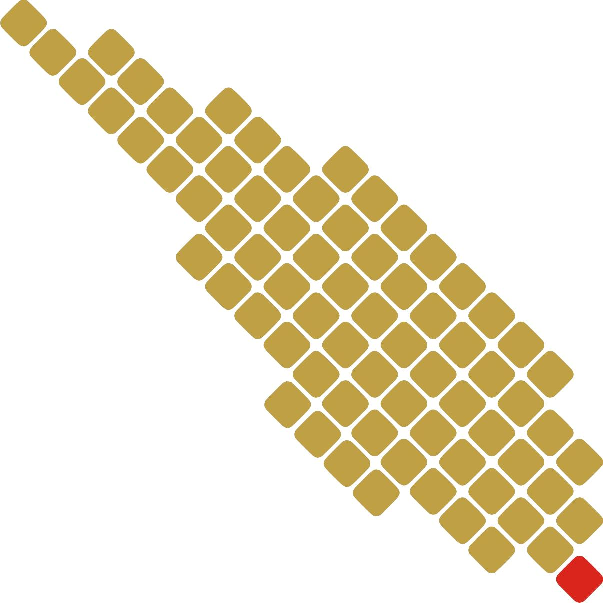
\includegraphics[width=3.2cm]{itera}\end{minipage}\hfill
\begin{minipage}{0.78\textwidth}
{\Large\bfseries Program Studi Matematika}\\[-1mm]
{\large Fakultas Sains}\\
{\large Institut Teknologi Sumatera}
\end{minipage}
\vspace{3mm}
{\color{enacom@color@gray}\rule{\textwidth}{1.2pt}}\\[-1mm]
{\color{enacom@color@blue}\rule{0.64\textwidth}{0.7pt}}
\vfill
{\Huge\bfseries Modul Praktikum\\[2mm] Pemodelan Komputasi dan Analisis Numerik}\par
\vspace{6mm}
{\Large MA25-31017}\par
\vspace{12mm}
{\large Disusun oleh}\par
\vspace{2mm}
{\Large Rifky Fauzi\\ Dear Michiko Mutiara Noor}\par
\vfill
{\color{enacom@color@blue}\rule{0.64\textwidth}{0.7pt}}\\[-1mm]
{\color{enacom@color@gray}\rule{\textwidth}{1.2pt}}
\vspace{3mm}
\begin{flushright}{\large Lampung Selatan, 2026}\end{flushright}
\end{titlepage}}
\AtBeginDocument{%
\pagestyle{fancy}%
\fancyhead{}%
\fancyhead[L]{\raisebox{-1mm}{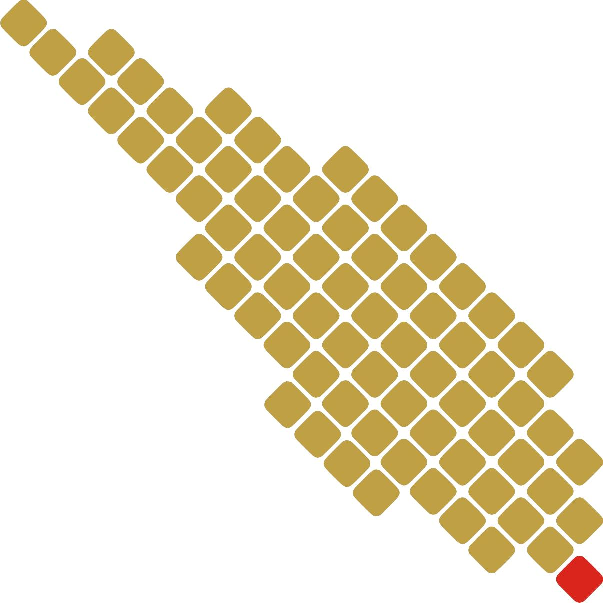
\includegraphics[height=8mm]{itera}}\hspace{2mm}\begin{minipage}[b]{0.72\textwidth}\small\bfseries \prodiheader\\[-1mm]\scriptsize Institut Teknologi Sumatera\end{minipage}}%
\fancyhead[R]{\scriptsize\thepage}%
\fancyfoot{}%
\fancyfoot[L]{\scriptsize \mkfooter}%
\fancyfoot[R]{\scriptsize Program Studi Matematika}%
\renewcommand{\headrulewidth}{0.6pt}%
\renewcommand{\footrulewidth}{0.4pt}%
\fancypagestyle{plain}{%
\fancyhead{}%
\fancyhead[L]{\raisebox{-1mm}{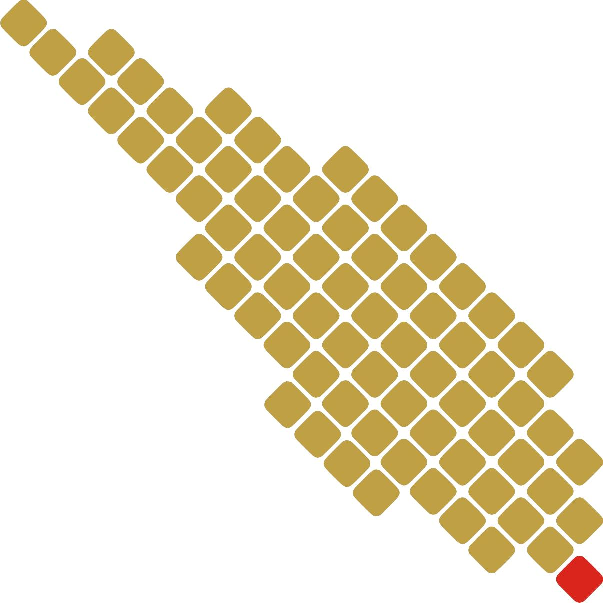
\includegraphics[height=8mm]{itera}}\hspace{2mm}\begin{minipage}[b]{0.72\textwidth}\small\bfseries \prodiheader\\[-1mm]\scriptsize Institut Teknologi Sumatera\end{minipage}}%
\fancyhead[R]{\scriptsize\thepage}%
\fancyfoot{}%
\fancyfoot[L]{\scriptsize \mkfooter}%
\fancyfoot[R]{\scriptsize Program Studi Matematika}%
\renewcommand{\headrulewidth}{0.6pt}%
\renewcommand{\footrulewidth}{0.4pt}%
}}
\makeatother


\begin{document}

\chapter*{Identitas Modul}
\addcontentsline{toc}{chapter}{Identitas Modul}
\begin{tabularx}{\textwidth}{>{\bfseries}p{0.28\textwidth}X}
Mata kuliah & Pemodelan Komputasi dan Analisis Numerik\\
Kode & MA25-31017\\
Program studi & Matematika\\
Fakultas & Fakultas Sains\\
Institusi & Institut Teknologi Sumatera\\
Perangkat lunak utama & MATLAB\\
Format pembelajaran & Praktikum, bedah jurnal, reproduksi komputasi, dan pembelajaran berbasis proyek\\
\end{tabularx}

\section*{Tentang modul}
Modul ini merupakan buku praktikum (bukan slide) untuk mata kuliah Pemodelan Komputasi dan Analisis Numerik. Struktur penyajian mengikuti pola modul praktikum: capaian, target luaran, materi singkat, algoritma, contoh, program MATLAB, verifikasi, dan latihan. Struktur praktikum terdiri atas sepuluh pertemuan terhitung. Seluruh butir pada Lembar Kerja/Bank Soal Praktikum B0.1--B7.5, Mock-Up UTS, dan Mock-Up UAS diintegrasikan kembali ke dalam contoh atau latihan modul dengan ID yang dipertahankan agar sinkron. Landasan teori utama modul menggunakan Chapra dan Canale, Numerical Methods for Engineers, edisi ke-7.

\section*{Capaian Pembelajaran Mata Kuliah (CPMK) utama}
\textbf{CPMK 6.1.} Mahasiswa mampu memecahkan (C4) masalah optimasi termasuk (dan tidak terbatas pada) masalah program linier, masalah pengujian hipotesis dan masalah pada proses stokastik dengan memilih (C3) model matematika yang sesuai, menerapkan (C3) langkah-langkah metode numerik yang terukur dan valid secara analitik untuk mendapatkan solusi, serta menginterpretasikan solusi yang diperoleh sesuai konteks masalah.

\textbf{CPMK 7.1.} Mahasiswa mampu merancang, menerapkan (C3), dan menganalisis (C4) model matematika berbasis metode numerik atau komputasi untuk memecahkan masalah di bidang sains, teknik, ekonomi, atau industri, serta mengevaluasi (C5) keakuratan, keterbatasan, dan relevansi model dalam konteks masalah nyata, dengan mendokumentasikan hasilnya secara ilmiah.

\section*{Peta praktikum}
\renewcommand{\arraystretch}{1.25}
\begin{tabularx}{\textwidth}{c c p{0.16\textwidth} X}
\hline
\textbf{Praktik} & \textbf{Minggu} & \textbf{Indikator} & \textbf{Fokus}\\\hline
1 & M2 & 6.1.1--6.1.3, 7.1.1 & Akar persamaan nonlinear: metode pengurungan dan metode terbuka\\
2 & M3 & 6.1.4 & Sistem Persamaan Linear (SPL) iteratif: Jacobi, Gauss-Seidel, residual, konvergensi\\
3 & M4 & 6.1.5, 7.1.1 & SPNL; regresi linear; pencocokan kurva nonlinear; MSE, RMSE, MAPE, dan $R^2$\\
4 & M5 & 6.1.6 & Turunan numerik: beda maju, beda mundur, beda pusat\\
5 & M6 & 6.1.7, 7.1.1 & Ukuran langkah, galat pemotongan, Richardson, reproduksi hasil\\
6 & M7 & 6.1.8 & Integral numerik: Trapezoid dan Simpson; pembanding Titik Tengah\\
7 & M9 & 6.1.9, 7.1.1 & Titik Tengah, Romberg, studi akurasi dan reproduksi artikel\\
8 & M10 & 6.1.10 & Masalah nilai awal: Euler dan evaluasi galat lokal/global\\
9 & M11 & 6.1.11, 7.1.1 & Runge-Kutta, stabilitas, ukuran langkah, reproduksi kurva model\\
10 & M12 & 6.1/7.1 & Praktikum terpadu: pemilihan metode, verifikasi dan validasi\\\hline
\end{tabularx}

\section*{Peta ketercakupan Lembar Kerja}
\renewcommand{\arraystretch}{1.18}
\begin{tabularx}{\textwidth}{p{0.24\textwidth}p{0.22\textwidth}X}
\hline
\textbf{Bagian Lembar Kerja} & \textbf{Lokasi dalam modul} & \textbf{Cakupan}\\\hline
B0.1--B0.5 & MATLAB Dasar & Variabel, kontrol alur, fungsi, grafik, galat, toleransi\\
B1.1--B1.5, B2.1--B2.5 & Praktikum 1 & Akar: grafik, Biseksi, Regula Falsi, Newton, Titik Tetap, Secant\\
B3.1--B3.5 & Praktikum 2 & SPL, solusi eksak, Jacobi, Gauss-Seidel, reaktor\\
B4.1--B4.5 & Praktikum 3 & SPNL; regresi linear; nonlinear curve fitting; MSE, RMSE, MAPE, $R^2$\\
B5.1--B5.4 & Praktikum 4 & Turunan analitik dan beda hingga\\
B5.5 & Praktikum 5 & Ukuran langkah dan sumber galat\\
B6.1--B6.3 & Praktikum 6 & Integral eksak, Trapezoid, Simpson\\
B6.4--B6.5 & Praktikum 7 & Integral komposit, refinement, evaluasi galat\\
B7.1--B7.2 & Praktikum 8 & Euler dan Heun\\
B7.3--B7.5 & Praktikum 9 & RK4, solusi eksak, perbandingan metode\\
UTS.1--UTS.4 & Lampiran Mock-Up UTS & Akar dan SPL\\
UAS.1--UAS.4 & Lampiran Mock-Up UAS & Turunan, integral, dan PDB\\\hline
\end{tabularx}

\chapter*{Petunjuk Umum Praktikum}
\addcontentsline{toc}{chapter}{Petunjuk Umum Praktikum}
\section*{Struktur setiap bab}
Setiap bab memuat enam komponen wajib: (1) capaian pembelajaran, (2) materi/teori, (3) algoritma, (4) contoh, (5) program MATLAB, dan (6) latihan. Naskah ini menambahkan tiga komponen yang disarankan untuk pembelajaran komputasi: \textit{target luaran}, \textit{checklist analisis}, dan \textit{verifikasi dan validasi}.

\section*{Sinkronisasi dengan Lembar Kerja}
Setiap soal pada Lembar Kerja Praktikum memiliki ID tetap (B0.1--B7.5, UTS.1--UTS.4, dan UAS.1--UAS.4). ID yang sama dipertahankan di modul. Dengan demikian, asisten dapat mengambil soal pre-test dari Lembar Kerja sementara mahasiswa dapat menemukan konsep, contoh, atau latihan yang relevan pada bab modul yang sesuai.

\section*{Prinsip pemrograman numerik}
\begin{enumerate}
\item Pisahkan \textit{skrip utama} dan fungsi numerik. Skrip utama memuat data, parameter, visualisasi, dan analisis; fungsi memuat algoritma.
\item Hindari invers matriks eksplisit. Di MATLAB, gunakan operator \texttt{\textbackslash} untuk menyelesaikan sistem linear.
\item Gunakan minimal dua kriteria berhenti ketika relevan: perubahan iterasi dan residual.
\item Selalu tetapkan \texttt{maxit} untuk mencegah loop tak berhingga.
\item Laporkan satuan, toleransi, ukuran langkah, jumlah iterasi, residual, dan metrik galat.
\item Pisahkan \textit{verifikasi} (apakah algoritma diimplementasikan benar?) dari \textit{validasi} (apakah model/hasil sesuai fenomena atau data?).
\end{enumerate}

\section*{Format ringkas laporan praktikum}
\begin{enumerate}
\item Tujuan dan capaian yang diuji.
\item Model/persamaan dan asumsi.
\item Metode numerik serta algoritma/pseudocode.
\item Implementasi MATLAB yang dapat direproduksi.
\item Verifikasi: kasus uji, residual, konvergensi, atau pembanding analitik.
\item Hasil: tabel dan grafik dengan label lengkap.
\item Analisis: pengaruh parameter numerik (toleransi, ukuran langkah, tebakan awal) dan keterbatasan.
\item Kesimpulan singkat berbasis hasil, bukan hanya mengulang teori.
\end{enumerate}



% ================================================================
\chapter{MATLAB Dasar}

\CP{Mahasiswa mampu menggunakan MATLAB untuk membuat variabel, percabangan, pengulangan, fungsi, dan grafik sederhana serta memahami ukuran galat sebelum menerapkannya pada algoritma numerik.}

\Target{Satu skrip MATLAB dasar yang memuat variabel, \texttt{if--else}, \texttt{for}/\texttt{while}, pemanggilan fungsi, tabel hasil, dan grafik sederhana.}

\section{Variabel dan operasi dasar}

MATLAB dapat digunakan sebagai kalkulator numerik sekaligus bahasa pemrograman.
Contoh paling dasar:

\begin{lstlisting}[language=Matlab]
clear; clc; close all

a = 1;
b = 1.5;
tol = 1e-6;
maxit = 100;

x = 0:0.1:2;
y = x.^3 - x - 1;
\end{lstlisting}

Untuk operasi elemen-per-elemen pada vektor gunakan
\texttt{.*}, \texttt{./}, dan \texttt{.\^}.

\section{Percabangan \texttt{if--else}}

Percabangan digunakan ketika program harus mengambil keputusan.

\begin{lstlisting}[language=Matlab]
f = @(x) x.^3 - x - 1;

if f(a)*f(b) < 0
    disp('Interval mengurung akar')
else
    disp('Belum ada perubahan tanda')
end
\end{lstlisting}

\section{Pengulangan}

\subsection*{\texttt{for}}

Gunakan \texttt{for} ketika jumlah pengulangan sudah diketahui.

\begin{lstlisting}[language=Matlab]
for k = 1:5
    fprintf('Iterasi ke-%d\n',k)
end
\end{lstlisting}

\subsection*{\texttt{while}}

Gunakan \texttt{while} ketika pengulangan bergantung pada suatu kondisi.

\begin{lstlisting}[language=Matlab]
err = 1;
k = 0;

while err > 1e-6 && k < 100
    k = k + 1;
    err = err/2;
end
\end{lstlisting}

\section{Membuat fungsi}

Fungsi dibuat agar algoritma dapat dipakai kembali.

\begin{lstlisting}[language=Matlab]
% File: nilaiF.m
function y = nilaiF(x)
    y = x.^3 - x - 1;
end
\end{lstlisting}

Kemudian dapat dipanggil dengan

\begin{lstlisting}[language=Matlab]
fx = nilaiF(1.25);
\end{lstlisting}

\section{Menggambar grafik sederhana}

Grafik berguna untuk melihat bentuk fungsi sebelum melakukan perhitungan numerik.

\begin{lstlisting}[language=Matlab]
x = linspace(0.5,1.7,300);
y = x.^3 - x - 1;

plot(x,y,'LineWidth',1.5)
yline(0,'--')
grid on
xlabel('x')
ylabel('f(x)')
title('Grafik f(x) = x^3 - x - 1')
\end{lstlisting}

Untuk grafik konvergensi, gunakan \texttt{semilogy} jika galat turun beberapa orde besaran.

\begin{lstlisting}[language=Matlab]
errs = [1e-1 4e-2 1.2e-2 3e-3 8e-4];
semilogy(1:numel(errs),errs,'o-')
grid on
xlabel('Iterasi')
ylabel('Galat')
title('Grafik konvergensi')
\end{lstlisting}

\section{Galat: definisi sebelum latihan}

Metode numerik menghasilkan hampiran. Karena itu ukuran galat harus didefinisikan sebelum digunakan.

Jika nilai sebenarnya $x^\ast$ diketahui, galat absolut adalah

\begin{equation}
E_t = |x^\ast-x_a|.
\end{equation}

Galat relatif sebenarnya adalah

\begin{equation}
\varepsilon_t =
\frac{|x^\ast-x_a|}{|x^\ast|},
\qquad x^\ast\neq0.
\end{equation}

Pada proses iterasi, nilai sebenarnya biasanya belum diketahui.
Gunakan perubahan relatif berskala

\begin{equation}
e_a^{(k)}
=
\frac{|x_{\mathrm{new}}-x_{\mathrm{old}}|}
{\max\left(1,|x_{\mathrm{new}}|\right)}.
\end{equation}

Bentuk ini tetap terdefinisi ketika $x_{\mathrm{new}}=0$ atau sangat dekat nol.
Jika ingin dinyatakan sebagai persen, gunakan $100e_a^{(k)}\%$.

Untuk vektor,

\begin{equation}
e_a^{(k)}
=
\max_i
\frac{|x_{i,\mathrm{new}}-x_{i,\mathrm{old}}|}
{\max\left(1,|x_{i,\mathrm{new}}|\right)}.
\end{equation}

Implementasi MATLAB:

\begin{lstlisting}[language=Matlab]
function e = relerr(xnew,xold)
    e = abs(xnew-xold)./max(1,abs(xnew));
end
\end{lstlisting}

\section{Latihan MATLAB Dasar}

\begin{enumerate}
\item Buat variabel \texttt{a}, \texttt{b}, \texttt{tol}, dan \texttt{maxit}, lalu tampilkan dengan \texttt{fprintf}.
\item Buat vektor $x=0:0.1:2$ dan hitung $f(x)=x^3-x-1$.
\item Gunakan \texttt{if--else} untuk memeriksa apakah $f(a)f(b)<0$.
\item Gunakan \texttt{for} untuk menghitung kuadrat bilangan 1 sampai 10.
\item Gunakan \texttt{while} yang berhenti jika galat lebih kecil dari $10^{-6}$.
\item Buat fungsi untuk $f(x)=x^3-x-1$.
\item Buat fungsi \texttt{relerr.m} berdasarkan formula perubahan relatif berskala di atas.
\item Gambar grafik $f(x)=x^3-x-1$ dan tambahkan garis $y=0$.
\item Buat grafik \texttt{semilogy} untuk suatu vektor \texttt{errs}.
\end{enumerate}

\section{Latihan fondasi dari Lembar Kerja}

\begin{enumerate}
\item[\textbf{B0.1 (L1)}] Jelaskan apa yang dimaksud dengan \textit{metode numerik}. Apa perbedaan utama antara solusi eksak/analitik dan solusi numerik?
\item[\textbf{B0.2 (L2)}] Nilai sebenarnya adalah \(x^\ast=\sqrt{3}\) dan hampiran yang diperoleh \(x_a=1.73\). Hitung galat absolut dan galat relatif sebenarnya.
\item[\textbf{B0.3 (L3)}] Suatu iterasi menghasilkan urutan hampiran \(2.0000,\ 1.7500,\ 1.7143,\ 1.7321\). Hitung perubahan relatif antariternasi dan bandingkan formula biasa dengan formula berskala yang menggunakan \(\max(1,|x_{\mathrm{new}}|)\).
\item[\textbf{B0.4 (L4)}] Jelaskan mengapa dua hampiran dapat mempunyai galat absolut yang sama tetapi kualitasnya berbeda. Kaitkan dengan galat relatif.
\item[\textbf{B0.5 (L5)}] Jelaskan peran \textit{round-off error}, \textit{truncation error}, toleransi, dan jumlah iterasi maksimum dalam algoritma numerik.
\end{enumerate}


\chapter{Praktikum 1: Akar Persamaan Nonlinear}

\CP{Mahasiswa mampu menerapkan Biseksi dan Regula Falsi sebagai metode pengurungan, memahami Titik Tetap, Newton-Raphson, dan Secant, serta mengevaluasi konvergensi menggunakan residual dan galat iterasi.}

\Target{Kode contoh kelas untuk Biseksi dan Regula Falsi, tabel iterasi, dan grafik konvergensi. Latihan utama dikerjakan dengan Biseksi, Newton-Raphson, dan Secant.}

\section{Masalah pencarian akar}

Tujuan pencarian akar adalah mencari $x$ sehingga

\begin{equation}
f(x)=0.
\end{equation}

Sebelum menghitung, gambar grafik untuk melihat posisi perubahan tanda dan memilih interval atau tebakan awal yang masuk akal.

Urutan metode dalam praktikum ini adalah:

\begin{enumerate}
\item Biseksi,
\item Regula Falsi,
\item Titik Tetap,
\item Newton-Raphson,
\item Secant.
\end{enumerate}

\section{Biseksi}

Jika $f$ kontinu pada $[a,b]$ dan

\begin{equation}
f(a)f(b)<0,
\end{equation}

maka sedikitnya satu akar berada di dalam interval.

Biseksi mengambil titik tengah

\begin{equation}
x_r=\frac{a+b}{2}.
\end{equation}

Kemudian interval diperbarui:

\begin{equation}
\begin{cases}
b\leftarrow x_r, & f(a)f(x_r)<0,\\
a\leftarrow x_r, & f(a)f(x_r)>0.
\end{cases}
\end{equation}

Galat iterasi yang dipakai:

\begin{equation}
e_a=
\frac{|x_{r,\mathrm{new}}-x_{r,\mathrm{old}}|}
{\max(1,|x_{r,\mathrm{new}}|)}.
\end{equation}

\subsection*{Langkah algoritma}

\begin{enumerate}
\item Pilih $a,b$ sehingga $f(a)f(b)<0$.
\item Hitung $x_r=(a+b)/2$.
\item Hitung $f(x_r)$ dan $e_a$.
\item Pilih interval baru berdasarkan tanda $f(a)f(x_r)$.
\item Ulangi sampai toleransi atau iterasi maksimum.
\end{enumerate}

\section{Regula Falsi}

Regula Falsi tetap memakai interval yang mengurung akar, tetapi kandidat akar tidak lagi menggunakan titik tengah.
Bangun garis yang melalui $(a,f(a))$ dan $(b,f(b))$.
Titik potong garis tersebut dengan sumbu-$x$ adalah

\begin{equation}
x_r
=
b-\frac{f(b)(b-a)}{f(b)-f(a)}
=
\frac{a f(b)-b f(a)}{f(b)-f(a)}.
\end{equation}

Setelah $x_r$ diperoleh, aturan pemilihan interval \textbf{sama dengan Biseksi}:

\begin{equation}
\begin{cases}
b\leftarrow x_r, & f(a)f(x_r)<0,\\
a\leftarrow x_r, & f(a)f(x_r)>0.
\end{cases}
\end{equation}

Jadi perbedaan inti kedua metode hanya terletak pada cara menghitung $x_r$.

\section{Titik Tetap}

Persamaan $f(x)=0$ diubah menjadi

\begin{equation}
x=g(x),
\end{equation}

kemudian dilakukan iterasi

\begin{equation}
x_{k+1}=g(x_k).
\end{equation}

Contoh:

\begin{equation}
e^{-x}-x=0
\qquad\Longrightarrow\qquad
x=e^{-x}.
\end{equation}

Syarat lokal sederhana untuk kecenderungan konvergen adalah

\begin{equation}
|g'(x^\ast)|<1.
\end{equation}

\section{Newton-Raphson}

Newton-Raphson menggunakan garis singgung pada titik $(x_k,f(x_k))$:

\begin{equation}
x_{k+1}
=
x_k-\frac{f(x_k)}{f'(x_k)}.
\end{equation}

Turunan harus ditentukan terlebih dahulu.

Contoh, untuk

\begin{equation}
f(x)=e^{-x}-x,
\end{equation}

diperoleh

\begin{equation}
f'(x)=-e^{-x}-1.
\end{equation}

\section{Secant}

Secant tidak memerlukan turunan analitik:

\begin{equation}
x_{k+1}
=
x_k-
f(x_k)
\frac{x_k-x_{k-1}}
{f(x_k)-f(x_{k-1})}.
\end{equation}

\section{Contoh kelas: Biseksi dan Regula Falsi}

Gunakan fungsi yang sama:

\begin{equation}
f(x)=x^3-x-1,
\qquad [a,b]=[1,1.5].
\end{equation}

Karena $f(1)=-1$ dan $f(1.5)=0.875$, interval mengurung akar.

Untuk Biseksi,

\begin{equation}
x_r=\frac{1+1.5}{2}=1.25.
\end{equation}

Untuk Regula Falsi,

\begin{equation}
x_r
=
1.5-\frac{0.875(1.5-1)}{0.875-(-1)}
\approx1.266667.
\end{equation}

Setelah nilai $x_r$ diperoleh, bagian kode yang memilih interval baru adalah identik.

\section{Program MATLAB yang dibahas di kelas}

Kode kelas hanya membandingkan Biseksi dan Regula Falsi.

\texttt{akar\_demo.m}

\lstinputlisting[language=Matlab]{matlab/akar_demo.m}

\section{Latihan / tugas utama}

\begin{enumerate}
\item \textbf{Biseksi.} Selesaikan $x^3-4x-9=0$. Tentukan interval sendiri, tampilkan tabel iterasi, simpan \texttt{errs}, dan gambar grafik konvergensi.
\item \textbf{Newton-Raphson.} Untuk $f(x)=e^{-x}-x$, tentukan $f'(x)$, gunakan sedikitnya dua tebakan awal, simpan \texttt{errs}, dan gambar grafik konvergensi.
\item \textbf{Secant.} Gunakan fungsi yang sama dengan Newton-Raphson, pilih dua tebakan awal, simpan \texttt{errs}, lalu bandingkan jumlah iterasi dan pola grafiknya dengan Newton-Raphson.
\end{enumerate}

\section{Latihan terintegrasi dari Lembar Kerja}

\begin{enumerate}
\item[\textbf{B1.1 (L1)}] Untuk \(f(x)=x^3-x-1\), buat tabel nilai \(f(x)\) untuk \(x=0.5,1,1.25,1.5,2\) dan tentukan interval yang masuk akal sebagai \textit{bracket}.
\item[\textbf{B1.2 (L2)}] Gunakan Biseksi untuk \(f(x)=x^3-x-1\) pada \([1,1.5]\). Lakukan 4 iterasi dan tuliskan tabel iterasinya.
\item[\textbf{B1.3 (L3)}] Gunakan Regula Falsi untuk fungsi yang sama dengan \(a=1\), \(b=1.5\). Lakukan 5 iterasi.
\item[\textbf{B1.4 (L4)}] Gunakan Newton-Raphson untuk \(f(x)=x^3-x-1\). Tentukan turunannya terlebih dahulu.
\item[\textbf{B1.5 (L5)}] Gunakan Newton-Raphson untuk \(f(x)=e^{-x}-x\). Tentukan turunannya, lakukan 5 iterasi, dan bandingkan konvergensinya dengan B1.4.
\item[\textbf{B2.1 (L1)}] Untuk \(e^{-x}-x=0\), gunakan \(g(x)=e^{-x}\) dan hitung 5 iterasi titik tetap dari \(x_0=0\).
\item[\textbf{B2.2 (L2)}] Evaluasi \(|g'(x^\ast)|\) di sekitar \(x^\ast\approx0.567\).
\item[\textbf{B2.3 (L3)}] Gunakan Secant untuk \(f(x)=e^{-x}-x\) dengan \(x_0=0\), \(x_1=1\), dan lakukan 5 pembaruan.
\item[\textbf{B2.4 (L4)}] Untuk \(\cos x-x=0\), tuliskan dua kemungkinan bentuk titik tetap dan diskusikan kecenderungan konvergensinya.
\item[\textbf{B2.5 (L5)}] Bandingkan Biseksi, Regula Falsi, Titik Tetap, Newton-Raphson, dan Secant dari kebutuhan tebakan awal, turunan, kecepatan, dan risiko divergensi.
\end{enumerate}


\chapter{Praktikum 2: Sistem Persamaan Linear Iteratif}

\CP{Mahasiswa mampu membangun algoritma Jacobi dan Gauss-Seidel dari bentuk persamaan skalar, kemudian menggunakan notasi matriks, mengevaluasi residual, galat, dan konvergensi.}

\Target{Implementasi Jacobi dan Gauss-Seidel, tabel iterasi, solusi pembanding, residual, dan grafik \texttt{errs}.}

\section{Mulai dari persamaan, bukan matriks}

Pertimbangkan tiga persamaan

\begin{align}
a_{11}x_1+a_{12}x_2+a_{13}x_3 &= b_1,\\
a_{21}x_1+a_{22}x_2+a_{23}x_3 &= b_2,\\
a_{31}x_1+a_{32}x_2+a_{33}x_3 &= b_3.
\end{align}

Masing-masing persamaan diselesaikan terhadap variabel diagonalnya:

\begin{align}
x_1 &=
\frac{b_1-a_{12}x_2-a_{13}x_3}{a_{11}},\\
x_2 &=
\frac{b_2-a_{21}x_1-a_{23}x_3}{a_{22}},\\
x_3 &=
\frac{b_3-a_{31}x_1-a_{32}x_2}{a_{33}}.
\end{align}

Dari bentuk inilah Jacobi dan Gauss-Seidel dibangun.

\section{Formula Jacobi}

Jacobi menggunakan seluruh nilai dari iterasi lama:

\begin{align}
x_1^{(k+1)}
&=
\frac{b_1-a_{12}x_2^{(k)}-a_{13}x_3^{(k)}}{a_{11}},\\
x_2^{(k+1)}
&=
\frac{b_2-a_{21}x_1^{(k)}-a_{23}x_3^{(k)}}{a_{22}},\\
x_3^{(k+1)}
&=
\frac{b_3-a_{31}x_1^{(k)}-a_{32}x_2^{(k)}}{a_{33}}.
\end{align}

Untuk $n$ variabel,

\begin{equation}
x_i^{(k+1)}
=
\frac{1}{a_{ii}}
\left(
b_i-\sum_{\substack{j=1\\j\ne i}}^n a_{ij}x_j^{(k)}
\right).
\end{equation}

\section{Formula Gauss-Seidel}

Gauss-Seidel langsung memakai nilai baru yang sudah tersedia:

\begin{align}
x_1^{(k+1)}
&=
\frac{b_1-a_{12}x_2^{(k)}-a_{13}x_3^{(k)}}{a_{11}},\\
x_2^{(k+1)}
&=
\frac{b_2-a_{21}x_1^{(k+1)}-a_{23}x_3^{(k)}}{a_{22}},\\
x_3^{(k+1)}
&=
\frac{b_3-a_{31}x_1^{(k+1)}-a_{32}x_2^{(k+1)}}{a_{33}}.
\end{align}

Untuk $n$ variabel,

\begin{equation}
x_i^{(k+1)}
=
\frac{1}{a_{ii}}
\left[
b_i
-\sum_{j=1}^{i-1}a_{ij}x_j^{(k+1)}
-\sum_{j=i+1}^{n}a_{ij}x_j^{(k)}
\right].
\end{equation}

Perbedaan utama:

\begin{itemize}
\item Jacobi: semua komponen memakai iterasi $k$.
\item Gauss-Seidel: komponen yang sudah dihitung langsung memakai iterasi $k+1$.
\end{itemize}

\section{Baru kemudian notasi matriks}

Sistem dapat diringkas menjadi

\begin{equation}
A\mathbf{x}=\mathbf{b}.
\end{equation}

Notasi matriks berguna untuk implementasi umum, tetapi algoritma di atas tetap berasal dari persamaan skalar.

\section{Galat iterasi dan residual}

Gunakan

\begin{equation}
e_a^{(k)}
=
\max_i
\frac{|x_i^{(k+1)}-x_i^{(k)}|}
{\max(1,|x_i^{(k+1)}|)}.
\end{equation}

Residual adalah

\begin{equation}
\mathbf{r}^{(k)}
=
\mathbf{b}-A\mathbf{x}^{(k)},
\end{equation}

dan salah satu ukuran residual adalah

\begin{equation}
r_k=\|\mathbf{r}^{(k)}\|_\infty.
\end{equation}

\section{Contoh}

Gunakan

\begin{align}
10x_1-x_2+2x_3&=6,\\
-x_1+11x_2-x_3&=25,\\
2x_1-x_2+10x_3&=-11.
\end{align}

Cari solusi eksak/analitik terlebih dahulu sebagai pembanding, lalu lakukan Jacobi dan Gauss-Seidel dari tebakan $(0,0,0)^T$.

\section{Program MATLAB}

\texttt{spl\_demo.m}

\lstinputlisting[language=Matlab]{matlab/spl_demo.m}

\section{Grafik konvergensi}

Simpan galat setiap iterasi pada vektor \texttt{errs}.

\begin{lstlisting}[language=Matlab]
semilogy(1:numel(errs),errs,'o-')
grid on
xlabel('Iterasi')
ylabel('e_a')
title('Grafik konvergensi')
\end{lstlisting}

Jika membandingkan Jacobi dan Gauss-Seidel, gambarkan kedua kurva pada satu grafik.

\section{Latihan}

\begin{enumerate}
\item Turunkan formula iterasi dari sistem persamaan, jangan mulai dari notasi matriks.
\item Tentukan solusi eksak/analitik sebagai pembanding.
\item Lakukan Jacobi dan Gauss-Seidel.
\item Hitung galat iterasi dan residual.
\item Simpan sejarah galat pada \texttt{errs}.
\item Buat grafik konvergensi kedua metode.
\item Jelaskan metode mana yang lebih cepat pada kasus tersebut.
\end{enumerate}

\section{Latihan terintegrasi dari Lembar Kerja}

\begin{enumerate}
\item[\textbf{B3.1 (L1)}] Tuliskan sistem \(10x_1-x_2+2x_3=6\), \(-x_1+11x_2-x_3=25\), \(2x_1-x_2+10x_3=-11\) ke bentuk \(A\mathbf{x}=\mathbf{b}\).
\item[\textbf{B3.2 (L2)}] Tentukan solusi eksak/analitik SPL tersebut.
\item[\textbf{B3.3 (L3)}] Gunakan Jacobi dari \((0,0,0)^T\), lakukan 3 iterasi, dan hitung galat setiap komponen.
\item[\textbf{B3.4 (L4)}] Gunakan Gauss-Seidel dari tebakan yang sama, lakukan 3 iterasi, lalu bandingkan dengan solusi eksak.
\item[\textbf{B3.5 (L5)}] Untuk model tiga reaktor, jelaskan pembentukan SPL dari neraca massa, susun bentuk matriksnya, dan tentukan solusi eksaknya.
\end{enumerate}


\chapter{Praktikum 3: SPNL dan Pencocokan Kurva}
\CP{Mahasiswa mampu menurunkan dan menjalankan Newton untuk beberapa variabel, merumuskan OLS linear sebagai SPL, membentuk Jacobian model nonlinear, menjalankan Gauss--Newton, dan mengevaluasi hasil dengan galat serta grafik konvergensi.}
\Target{Dua bagian terpisah: SPNL dan pencocokan kurva. Kode terdiri atas fungsi algoritma yang dapat digunakan ulang dan \emph{driver} berisi data, parameter, tabel, serta visualisasi.}

\section{Bagian A --- Newton untuk Sistem Persamaan Nonlinear}
\subsection{Dari akar skalar ke beberapa variabel}
Pada satu variabel, Newton mencari akar $f(x)=0$ dengan menggunakan turunan $f'(x)$. Pada $n$ variabel, kita mencari vektor $\mathbf{x}=(x_1,\ldots,x_n)^T$ yang membuat \emph{seluruh} persamaan bernilai nol:
\begin{equation}
\mathbf{F}(\mathbf{x})=\begin{bmatrix}f_1(\mathbf{x})\\ \vdots\\ f_n(\mathbf{x})\end{bmatrix}=\mathbf{0}.
\end{equation}
Turunan $f'(x)$ digantikan oleh \textbf{matriks Jacobian}, yaitu kumpulan turunan parsial:
\begin{equation}
J_F(\mathbf{x})=\left[\frac{\partial f_i}{\partial x_j}(\mathbf{x})\right]_{i,j=1}^{n}.
\end{equation}
Jangan mencampurkan nama \emph{matriks Jacobian} ($J_F$) dengan metode \emph{Jacobi} pada SPL: keduanya berbeda.

\subsection{Penurunan Newton multivariabel}
Linearisasi Taylor orde pertama di titik $\mathbf{x}^{(k)}$ menghasilkan
\begin{equation}
\mathbf{F}(\mathbf{x}^{(k)}+\Delta\mathbf{x})\approx
\mathbf{F}(\mathbf{x}^{(k)})+J_F(\mathbf{x}^{(k)})\Delta\mathbf{x}.
\end{equation}
Kita meminta model linear ini sama dengan nol. Akibatnya, \textbf{setiap iterasi Newton menyelesaikan SPL}:
\begin{align}
J_F(\mathbf{x}^{(k)})\Delta\mathbf{x}^{(k)}&=-\mathbf{F}(\mathbf{x}^{(k)}),\\
\mathbf{x}^{(k+1)}&=\mathbf{x}^{(k)}+\Delta\mathbf{x}^{(k)}.
\end{align}
Di MATLAB gunakan \texttt{delta = -J(z)\textbackslash F(z)}, bukan menghitung \texttt{inv(J)}.

\subsection{Algoritma Newton multivariabel}
\begin{enumerate}
\item Tentukan $\mathbf{F}$, Jacobian $J_F$, tebakan awal $\mathbf{x}^{(0)}$, toleransi $\tau$, dan batas iterasi $N_{\max}$.
\item Pada iterasi $k$, hitung $\mathbf{F}_k=\mathbf{F}(\mathbf{x}^{(k)})$ dan $J_k=J_F(\mathbf{x}^{(k)})$.
\item Pastikan Jacobian tidak singular/nyaris singular; selesaikan SPL $J_k\Delta\mathbf{x}^{(k)}=-\mathbf{F}_k$.
\item Perbarui $\mathbf{x}^{(k+1)}=\mathbf{x}^{(k)}+\Delta\mathbf{x}^{(k)}$. Jika langkah penuh memperbesar residual, coba langkah teredam atau ubah tebakan awal.
\item Simpan galat perubahan relatif berskala dan residual:
\begin{equation}
 e_k=\max_i\frac{|x_i^{(k+1)}-x_i^{(k)}|}{\max(1,|x_i^{(k+1)}|)},
 \qquad r_k=\|\mathbf{F}(\mathbf{x}^{(k+1)})\|_\infty.
\end{equation}
\item Hentikan jika kriteria yang dipilih terpenuhi; laporkan \emph{kedua} ukuran dan status bila $N_{\max}$ tercapai.
\end{enumerate}
\Note{Tebakan awal adalah \emph{educated guess}, bukan harus angka tertentu. Patuhi domain model (misalnya konsentrasi positif), lihat grafik/arti variabel, dan hindari tebakan pada Jacobian singular. Newton lokal tidak menjamin konvergensi dari sebarang tebakan.}

\subsection{Contoh terhitung}
Tentukan penyelesaian
\begin{align}
f_1(x,y)&=x^2+y^2-5=0,\\
f_2(x,y)&=x-y-1=0.
\end{align}
Dengan $\mathbf{x}^{(0)}=(1.5,0.5)^T$, diperoleh
\begin{equation}
\mathbf{F}(\mathbf{x}^{(0)})=\begin{bmatrix}-2.5\\0\end{bmatrix},\qquad
J_F(\mathbf{x}^{(0)})=\begin{bmatrix}3&1\\1&-1\end{bmatrix}.
\end{equation}
Selesaikan $J_F\Delta\mathbf{x}=-\mathbf{F}$ untuk memperoleh $\Delta\mathbf{x}=(0.625,0.625)^T$; jadi $\mathbf{x}^{(1)}=(2.125,1.125)^T$. Lanjutkan sampai residual kecil. Periksa solusi analitik $(2,1)$ dan $(-1,-2)$: sistem ini mempunyai lebih dari satu akar.

\subsection{Pisahkan function dan driver}
\textbf{Function:} \texttt{newton\_spnl.m} memuat algoritma dan \texttt{history}. \textbf{Driver:} \texttt{driver\_spnl.m} menetapkan persamaan, Jacobian, tebakan awal, tabel, serta grafik.
\MatlabFile{newton\_spnl.m (function)}
\lstinputlisting[language=Matlab]{matlab/newton_spnl.m}
\MatlabFile{driver\_spnl.m (driver)}
\lstinputlisting[language=Matlab]{matlab/driver_spnl.m}

\subsection{Latihan SPNL}
\begin{enumerate}
\item Turunkan $J_F$ sendiri sebelum menjalankan kode; hitung satu iterasi manual.
\item Jalankan dari tiga tebakan awal dan identifikasi solusi yang diperoleh; perhatikan domain yang relevan.
\item Buat \texttt{semilogy} untuk \texttt{history.errs} dan \texttt{history.residual}; jelaskan jika suatu grafik stagnan.
\item Modifikasi driver untuk sistem lain, sedangkan function Newton tetap sama.
\end{enumerate}

\section{Bagian B --- Regresi linear dan nonlinear}
\subsection{Data dan definisi dua model}
Pada contoh kelas, gunakan \textbf{data yang sama} untuk kedua model:
\begin{center}
\begin{tabular}{c|ccccc}\hline
$x_i$&0.25&0.75&1.25&1.75&2.25\\
$y_i$&0.28&0.57&0.68&0.74&0.79\\\hline
\end{tabular}
\end{center}
Model linear: $\widehat y_i=a+b x_i$. Model nonlinear (saturasi sesuai contoh kelas):
\begin{equation}
\widehat y_i=f(x_i;\mathbf{a})=a_0\bigl(1-e^{-a_1x_i}\bigr),
\qquad \mathbf{a}=(a_0,a_1)^T,\quad \mathbf{a}^{(0)}=(1,1)^T.
\label{eq:model_saturasi}
\end{equation}
Model linear mempunyai koefisien linear dalam parameter. Model saturasi nonlinear dalam parameter $a_1$, sehingga membutuhkan iterasi untuk mendapatkan nilai least squares.

\subsection{Regresi linear: dari OLS sampai SPL}
Residual $r_i=y_i-(a+bx_i)$. \emph{Ordinary least squares} (OLS) meminimalkan
\begin{equation}
S(a,b)=\sum_{i=1}^n\bigl[y_i-a-bx_i\bigr]^2.
\end{equation}
Setel kedua turunan parsial objektif ke nol:
\begin{align}
\frac{\partial S}{\partial a}&=-2\sum_i(y_i-a-bx_i)=0,\\
\frac{\partial S}{\partial b}&=-2\sum_ix_i(y_i-a-bx_i)=0.
\end{align}
Diperoleh SPL \emph{normal equations}:
\begin{equation}
\underbrace{\begin{bmatrix}n&\sum x_i\\\sum x_i&\sum x_i^2\end{bmatrix}}_{X^TX}
\underbrace{\begin{bmatrix}a\\b\end{bmatrix}}_{\boldsymbol\beta}
=\underbrace{\begin{bmatrix}\sum y_i\\\sum x_i y_i\end{bmatrix}}_{X^T\mathbf{y}},\quad
X=\begin{bmatrix}1&x_1\\\vdots&\vdots\\1&x_n\end{bmatrix}.
\label{eq:linear_normal}
\end{equation}
Untuk data kelas,
\begin{equation}
\begin{bmatrix}5&6.25\\6.25&10.3125\end{bmatrix}
\begin{bmatrix}a\\b\end{bmatrix}
=\begin{bmatrix}3.06\\4.42\end{bmatrix},\qquad
\widehat{\boldsymbol\beta}=\begin{bmatrix}0.3145\\0.2380\end{bmatrix}.
\end{equation}
Dalam perangkat lunak, \texttt{X\textbackslash y} menyelesaikan OLS lebih stabil daripada \texttt{inv(X'*X)*X'*y}; persamaan normal dipakai untuk \textbf{memahami formulasi}, bukan perintah wajib menghitung invers.
\MatlabFile{regresi\_linear.m (function)}
\lstinputlisting[language=Matlab]{matlab/regresi_linear.m}

\subsection{Regresi nonlinear: fungsi, Jacobian, dan pembaruan parameter}
Untuk model \eqref{eq:model_saturasi}, residual dan objektifnya ialah
\begin{equation}
D_i(\mathbf{a})=y_i-f(x_i;\mathbf{a}),\qquad
S(\mathbf{a})=\tfrac12\sum_iD_i(\mathbf{a})^2.
\end{equation}
Turunan parsial \textbf{model terhadap parameter}:
\begin{align}
\frac{\partial f}{\partial a_0}&=1-e^{-a_1x},\\
\frac{\partial f}{\partial a_1}&=a_0x e^{-a_1x}.
\end{align}
Susun Jacobian model $Z\in\mathbb{R}^{n\times2}$ dengan baris
\begin{equation}
Z_{i,:}(\mathbf{a})=
\begin{bmatrix}1-e^{-a_1x_i}&a_0x_i e^{-a_1x_i}\end{bmatrix}.
\end{equation}
Di $\mathbf{a}^{(0)}=(1,1)^T$ berlaku (pembulatan empat desimal):
\begin{equation}
Z_0=\begin{bmatrix}
0.2212&0.1947\\0.5276&0.3543\\0.7135&0.3581\\0.8262&0.3041\\0.8946&0.2371
\end{bmatrix},\qquad
\mathbf{D}_0=\begin{bmatrix}0.0588\\0.0424\\-0.0335\\-0.0862\\-0.1046\end{bmatrix}.
\label{eq:class_Z_D}
\end{equation}
Ini adalah matriks dan residual pada \textbf{gambar contoh kelas}; nilai lengkap tanpa pembulatan digunakan dalam program.

\subsection{Menurunkan algoritma Gauss--Newton}
Linearisasi model $f(\mathbf{a}+\Delta\mathbf{a})\approx f(\mathbf{a})+Z\Delta\mathbf{a}$ menghasilkan
\begin{equation}
\mathbf{D}(\mathbf{a}+\Delta\mathbf{a})\approx\mathbf{D}-Z\Delta\mathbf{a}.
\end{equation}
Cari $\Delta\mathbf{a}$ yang meminimalkan $\|\mathbf{D}-Z\Delta\mathbf{a}\|_2^2$. Persamaan normal untuk langkah adalah
\begin{equation}
\underbrace{(Z^TZ)}_{2\times2}\Delta\mathbf{a}=Z^T\mathbf{D},
\label{eq:gn_normal}
\end{equation}
lalu perbarui parameter:
\begin{equation}
\mathbf{a}^{(k+1)}=\mathbf{a}^{(k)}+\alpha_k\Delta\mathbf{a}^{(k)},\qquad 0<\alpha_k\le1.
\label{eq:gn_update}
\end{equation}
Secara numerik, implementasi \texttt{delta = Z\textbackslash D} memecahkan masalah least squares tanpa membentuk $Z^TZ$ secara eksplisit. \texttt{alpha} dapat dibagi dua bila objektif justru membesar. Untuk data contoh, langkah penuh pertama sekitar $\Delta\mathbf{a}=(-0.27148,\,0.50193)^T$.

\subsection{Algoritma fungsi regresi nonlinear}
\begin{enumerate}
\item Input $x,y$, model $f(x;\mathbf{a})$, Jacobian model $Z(x,\mathbf{a})$, tebakan awal, toleransi dan batas iterasi.
\item Evaluasi vektor residual $\mathbf{D}=\mathbf{y}-\widehat{\mathbf{y}}$ dan Jacobian $Z$ berukuran $n\times p$.
\item Periksa dimensi dan rank, lalu selesaikan masalah least squares $Z\Delta\mathbf{a}\approx\mathbf{D}$ (ekuivalen dengan \eqref{eq:gn_normal} bila rank penuh).
\item Uji parameter $\mathbf{a}+\alpha\Delta\mathbf{a}$; kurangi $\alpha$ jika SSE membesar.
\item Catat parameter, \texttt{errs} dan SSE untuk grafik; ulangi sampai toleransi atau iterasi maksimum.
\item Periksa kewajaran parameter, pola residual dan kualitas hasil; perubahan parameter kecil saja tidak membuktikan kecocokan data baik.
\end{enumerate}
\MatlabFile{regresi\_nonlinear.m (function)}
\lstinputlisting[language=Matlab]{matlab/regresi_nonlinear.m}
\MatlabFile{driver\_regresi.m (driver)}
\lstinputlisting[language=Matlab]{matlab/driver_regresi.m}

\subsection{Evaluasi model dan grafik}
Dengan $r_i=y_i-\widehat y_i$, $\bar y=\frac1n\sum_i y_i$, dan $\mathrm{SSE}=\sum r_i^2$:
\begin{align}
\mathrm{MSE}&=\frac1n\sum_i r_i^2, &
\mathrm{RMSE}&=\sqrt{\mathrm{MSE}},\\
\mathrm{MAPE}&=\frac{100}{n}\sum_i\left|\frac{r_i}{y_i}\right|, &
R^2&=1-\frac{\mathrm{SSE}}{\sum_i(y_i-\bar y)^2}.
\end{align}
MAPE klasik tidak terdefinisi untuk $y_i=0$; $R^2$ tidak terdefinisi jika seluruh $y_i$ sama. Jangan menuliskan hasil metrik tanpa memeriksa kondisi tersebut. \texttt{driver\_regresi.m} menghasilkan grafik titik data dan kedua model, grafik residual, serta \texttt{semilogy} galat parameter per iterasi.

\section{Latihan terintegrasi dari Lembar Kerja}
\begin{enumerate}
\item[\textbf{B4.1 (L1)}] Susun $x^2+y^2-5=0$ dan $x-y-1=0$ dalam bentuk vektor $\mathbf{F}(x,y)=\mathbf{0}$. Jelaskan hubungan dengan pencarian akar skalar.
\item[\textbf{B4.2 (L2)}] Tentukan Jacobian $J_F(x,y)$ dan daerah di mana Jacobian tidak invertibel.
\item[\textbf{B4.3 (L3)}] Mulai dari $(1.5,0.5)$, kerjakan satu langkah Newton multivariabel secara manual, lalu cocokkan dengan \texttt{driver\_spnl.m}.
\item[\textbf{B4.4 (L4, di kelas)}] Sesuai Lembar Kerja, gunakan data $ (1,0.5),(2,2.5),(3,2.0),(4,4.0),(5,3.5)$. (a) Cari model regresi linear $\widehat y=a+bx$ dengan OLS, turunkan SPL normalnya. (b) \textbf{Tambahan nonlinear:} pada \emph{data yang sama} fit $\widehat y=a_0(1-e^{-a_1x})$, bentuk Jacobian parameter $Z$, lalu jalankan Gauss--Newton. (c) Hitung MSE, RMSE, MAPE, $R^2$ dan buat grafik data-model, residual serta \texttt{errs}. Bandingkan pula dengan contoh data kelas di bagian sebelumnya.
\item[\textbf{B4.5 (L5, tugas)}] Gunakan dua belas data saturasi pada tabel berikut. Model \textbf{default} adalah $\widehat y=a_0(1-e^{-a_1x})$. Hitung parameter dan keempat metrik serta grafik \texttt{errs}. Untuk tantangan, coba model saturasi rasional $\widehat y=c_0x/(c_1+x)$ pada \textbf{data yang sama}; turunkan Jacobian parameter dan bandingkan metriknya. Jelaskan perbedaan bentuk model dan batasan parameter. Untuk mempertahankan butir asli B4.5, tuliskan juga objektif $S(a,b)=\sum_i(y_i-ae^{bx_i})^2$ dan kondisi optimalitas $\partial_a S=\partial_b S=0$ untuk model eksponensial $ae^{bx}$.
\end{enumerate}
\begin{center}\small
\begin{tabular}{c|rrrrrr}\hline
$x$&0.25&0.75&1.25&1.75&2.25&2.75\\
$y$&0.165&0.440&0.612&0.771&0.859&0.945\\\hline
$x$&3.25&3.75&4.25&4.75&5.25&5.75\\
$y$&0.988&1.044&1.065&1.097&1.102&1.118\\\hline
\end{tabular}
\end{center}
\Note{Data tugas adalah data sintetis pembelajaran, bukan hasil pengukuran lapangan. Bila ingin mencoba model eksponensial tumbuh $\widehat y=ae^{bx}$, gunakan dataset tambahan dalam \texttt{matlab/data\_eksponensial.csv}; model itu \emph{tidak} mempunyai plateau dan karena itu tidak otomatis cocok untuk data saturasi. Untuk dua parameter $a,b$, turunan Jacobian-nya adalah $\partial f/\partial a=e^{bx}$ dan $\partial f/\partial b=ax e^{bx}$.}

\subsection*{Dataset opsional: pertumbuhan eksponensial (12 titik)}
Untuk mahasiswa yang ingin mencoba fungsi $\widehat y=ae^{bx}$ dari butir awal B4.5, gunakan data sintetis \emph{berbeda} berikut, bukan data saturasi di atas:
\begin{center}\small
\begin{tabular}{c|rrrrrr}\hline
$x$&0.5&1.0&1.5&2.0&2.5&3.0\\
$y$&0.806&0.920&1.159&1.410&1.641&2.057\\\hline
$x$&3.5&4.0&4.5&5.0&5.5&6.0\\
$y$&2.488&2.932&3.604&4.366&5.235&6.395\\\hline
\end{tabular}
\end{center}
Fit $f(x;a,b)=ae^{bx}$ dengan Jacobian model $Z_i=[e^{bx_i},\; ax_i e^{bx_i}]$. Sebagai tantangan lain, bandingkan dengan fungsi pangkat $f(x;c,d)=cx^d$ (untuk $x>0$), dengan turunan parameter $\partial_c f=x^d$ dan $\partial_d f=cx^d\ln x$. Hitung empat metrik pada \textbf{data yang sama} dan gambarkan \texttt{errs}. Jangan menggabungkan dataset pertumbuhan ini dengan dataset saturasi pada satu fitting.

\section{Tugas refleksi komputasi}
Jalankan seluruh driver dengan data sesuai instruksi. Jelaskan isi input/output tiap function, tunjukkan apa yang berubah ketika tebakan awal diganti, serta simpan grafik \texttt{errs} dan residual dengan label lengkap.


\chapter{Praktikum 4: Turunan Numerik dengan Beda Hingga}
\CP{Mahasiswa mampu menerapkan beda maju, beda mundur, dan beda pusat serta menjelaskan orde akurasi turunan numerik (indikator 6.1.6).}
\Target{Fungsi MATLAB generik untuk tiga skema beda hingga, tabel galat terhadap ukuran langkah, dan grafik log-log yang menunjukkan perbedaan orde akurasi.}

\section{Materi singkat dan landasan teori}
Beda hingga diturunkan dari ekspansi Taylor. Untuk $h>0$,
\begin{align}
f(x+h)&=f(x)+hf'(x)+\frac{h^2}{2}f''(x)+O(h^3),\\
f(x-h)&=f(x)-hf'(x)+\frac{h^2}{2}f''(x)+O(h^3).
\end{align}
Dari persamaan pertama diperoleh beda maju
\begin{equation}
f'(x)\approx\frac{f(x+h)-f(x)}{h}=f'(x)+O(h).
\end{equation}
Beda mundur juga berorde satu. Dengan mengurangkan dua ekspansi Taylor diperoleh beda pusat
\begin{equation}
f'(x)\approx\frac{f(x+h)-f(x-h)}{2h}=f'(x)+O(h^2).
\end{equation}
Karena itu, ketika $h$ dibagi dua, galat pemotongan beda maju idealnya turun sekitar faktor 2, sedangkan beda pusat sekitar faktor 4, selama pembulatan belum dominan.

Ukuran langkah tidak boleh dipilih sekecil mungkin tanpa batas. Ketika $h$ terlalu kecil, pengurangan dua bilangan yang hampir sama menyebabkan pembatalan numerik dan pembulatan galat dapat membesar. Secara praktis terdapat wilayah dominasi galat pemotongan, wilayah optimum, dan wilayah dominasi pembulatan.

\section{Algoritma}
\begin{enumerate}
\item Tetapkan $f$, titik $x_0$, dan daftar $h$.
\item Untuk setiap $h$, hitung beda maju, mundur, dan pusat.
\item Jika solusi analitik tersedia, hitung galat absolut/relatif. Jika tidak, gunakan solusi referensi berakurasi lebih tinggi secara hati-hati.
\item Plot galat terhadap $h$ pada skala log-log.
\item Estimasikan kemiringan grafik untuk mengamati orde akurasi.
\end{enumerate}

\section{Contoh}
Ambil
\begin{equation}
f(x)=\frac{e^x}{\sin(\sqrt{x})},\qquad x_0=1.2.
\end{equation}
Turunan analitik pada $x_0$ sekitar $2.85683778241$. Dengan $h=0.1$, beda pusat memberikan sekitar $2.86120081209$, jauh lebih akurat daripada beda maju/mundur pada step yang sama. Ketika $h$ dibagi dua berulang kali, galat beda pusat menunjukkan orde mendekati dua sebelum efek pembulatan muncul.

\section{Program MATLAB}
\lstinputlisting[language=Matlab]{matlab/finite_difference.m}
\lstinputlisting[language=Matlab]{matlab/numdiff.m}

\AnalysisCheck{Jangan hanya melaporkan nilai turunan. Tunjukkan hubungan $h$-galat dan jawab: skema mana paling akurat pada biaya evaluasi fungsi yang sebanding?}

\section{Latihan}
\begin{enumerate}
\item Turunkan sendiri formula beda pusat dari deret Taylor.
\item Uji $f(x)=\sin(1/x)$ pada $x=0.4$ untuk beberapa $h$. Jelaskan mengapa fungsi yang berosilasi cepat menuntut kehati-hatian.
\item Estimasikan orde observasi dengan $p\approx\log(E_h/E_{h/2})/\log 2$.
\item Buat fungsi untuk hampiran turunan kedua dengan beda pusat dan uji pada $f(x)=e^x$.

\item Ulangi percobaan dengan toleransi atau ukuran langkah yang berbeda, lalu jelaskan apakah kesimpulan berubah.
\item Tambahkan satu grafik pendukung dan beri judul, label sumbu, legenda, serta penjelasan singkat.
\item Susun satu paragraf interpretasi hasil: apa yang berhasil, apa keterbatasannya, dan parameter numerik mana yang paling berpengaruh.

\end{enumerate}

% ================================================================
\section{Latihan terintegrasi dari Lembar Kerja}
Untuk setiap fungsi, tentukan turunan analitik terlebih dahulu agar galat sebenarnya dapat dievaluasi.
\begin{enumerate}
\item[\textbf{B5.1 (L1)}] Untuk \(f(x)=x\sqrt{x}-7x\), tentukan turunan analitik \(f'(x)\).
\item[\textbf{B5.2 (L2)}] Gunakan beda maju, beda mundur, dan beda pusat dengan \(h=0.5\) untuk menghampiri \(f'(1.5)\) pada fungsi B5.1.
\item[\textbf{B5.3 (L3)}] Hitung nilai eksak \(f'(1.5)\) dari hasil soal B5.1, kemudian tentukan galat absolut dan galat relatif sebenarnya untuk ketiga hampiran pada B5.2.
\item[\textbf{B5.4 (L4)}] Untuk fungsi \(f(x)=\ln x\), tentukan turunan analitik \(f'(x)\), lalu hampiri \(f'(2)\) dengan beda pusat menggunakan \(h=0.25\). Evaluasi galat relatif sebenarnya.
\end{enumerate}

\chapter{Praktikum 5: Ukuran Langkah, Galat Pemotongan, dan Richardson}
\CP{Mahasiswa mampu menganalisis pengaruh ukuran langkah dan galat pemotongan pada turunan numerik serta mereproduksi hasil komputasi dari sumber ilmiah (indikator 6.1.7 dan 7.1.1).}
\Target{Eksperimen konvergensi yang menunjukkan orde metode, ekstrapolasi Richardson, dan pembahasan wilayah optimum ukuran langkah.}

\section{Materi singkat dan landasan teori}
Misalkan aproksimasi $D(h)$ memiliki ekspansi galat
\begin{equation}
D(h)=D^*+C h^p+O(h^{p+1}),
\end{equation}
dengan $p$ orde utama. Evaluasi pada $h$ dan $h/2$ dapat dikombinasikan untuk mengeliminasi suku $Ch^p$:
\begin{equation}
D_R=D(h/2)+\frac{D(h/2)-D(h)}{2^p-1}.
\end{equation}
Inilah ide Richardson ekstrapolasi. Untuk beda pusat $p=2$, penyebutnya $2^2-1=3$. Metode ini meningkatkan orde tanpa harus menurunkan formula baru dari awal.

Analisis konvergensi eksperimental sangat penting pada artikel komputasi. Jika solusi eksak $D^*$ tersedia, hitung $E_h=|D(h)-D^*|$. Jika tidak tersedia, bandingkan perhalusan berturut-turut atau solusi referensi yang jauh lebih halus. Orde observasi dapat diperkirakan
\begin{equation}
p_{obs}=\frac{\log(E_h/E_{h/2})}{\log 2}.
\end{equation}
Nilai $p_{obs}$ mendekati orde teori hanya pada rentang asimtotik. Jika terlalu kasar, higher-order terms masih dominan; jika terlalu kecil, pembulatan dapat merusak pola.

\section{Algoritma}
\begin{enumerate}
\item Pilih skema dasar dengan orde $p$ dan urutan $h_j=h_0/2^j$.
\item Hitung $D(h_j)$ dan $D(h_j/2)$.
\item Bentuk $D_R$ dan galat terhadap referensi.
\item Plot galat terhadap $h$ secara log-log dan hitung $p_{obs}$.
\item Tandai wilayah di mana galat berhenti turun.
\end{enumerate}

\section{Contoh}
Untuk fungsi pada Praktikum 4 dan $x_0=1.2$, beda pusat dengan $h=0.2$ memberi sekitar $2.87423645$ dan dengan $h=0.1$ sekitar $2.86120081$. Richardson menghasilkan sekitar $2.85685560$, sangat dekat dengan nilai analitik $2.85683778$.

\section{Program MATLAB}
\lstinputlisting[language=Matlab]{matlab/richardson_diff.m}

\section{Latihan}
\begin{enumerate}
\item Terapkan Richardson pada beda maju ($p=1$) dan bandingkan dengan beda pusat biasa.
\item Gunakan $h$ dari $10^{-1}$ sampai $10^{-12}$. Identifikasi titik ketika pembulatan mulai mendominasi.
\item Ambil satu figur/tabel turunan numerik dari artikel dan reproduksi minimal satu hasilnya. Catat semua parameter numerik yang harus diasumsikan karena tidak dilaporkan.
\item Diskusikan mengapa reproduksi hasil merupakan bagian dari verifikasi, bukan otomatis validasi model.

\item Ulangi percobaan dengan toleransi atau ukuran langkah yang berbeda, lalu jelaskan apakah kesimpulan berubah.
\item Tambahkan satu grafik pendukung dan beri judul, label sumbu, legenda, serta penjelasan singkat.
\item Susun satu paragraf interpretasi hasil: apa yang berhasil, apa keterbatasannya, dan parameter numerik mana yang paling berpengaruh.

\end{enumerate}

% ================================================================
\section{Latihan lanjutan dari Lembar Kerja}
\begin{enumerate}
\item[\textbf{B5.5 (L5)}] Jelaskan mengapa pemilihan \(h\) yang terlalu besar maupun terlalu kecil dapat menghasilkan kesalahan besar pada turunan numerik. Kaitkan dengan \textit{truncation error} dan \textit{round-off error}.
\end{enumerate}

\chapter{Praktikum 6: Integral Numerik Dasar}
\CP{Mahasiswa mampu menerapkan aturan Trapezoid dan Simpson serta mengevaluasi galat integrasi numerik (indikator 6.1.8).}
\Target{Implementasi Trapezoid, Titik Tengah, dan Simpson komposit, studi jejaring perhalusan, serta perbandingan orde galat.}

\section{Materi singkat dan landasan teori}
Integral tentu dapat dihampiri dengan mengintegralkan interpolan polinomial. Aturan Trapezoid memakai interpolan linear pada setiap subinterval. Untuk jejaring seragam $h=(b-a)/n$,
\begin{equation}
I_T=h\left[\frac12f(x_0)+\sum_{i=1}^{n-1}f(x_i)+\frac12f(x_n)\right],
\end{equation}
dengan galat global $O(h^2)$ untuk fungsi cukup mulus.

Aturan Titik Tengah juga berorde dua:
\begin{equation}
I_M=h\sum_{i=1}^{n} f\left(a+\left(i-\frac12\right)h\right).
\end{equation}
Aturan Simpson 1/3 mengintegralkan interpolan kuadratik dan, untuk $n$ genap,
\begin{equation}
I_S=\frac{h}{3}\left[f_0+f_n+4\sum_{i\;ganjil}f_i+2\sum_{i\;genap,\,i\ne 0,n}f_i\right],
\end{equation}
dengan galat global $O(h^4)$.

\section{Algoritma}
\begin{enumerate}
\item Pilih $n$, hitung $h=(b-a)/n$ dan titik grid.
\item Evaluasi $f$ secara vektor bila memungkinkan.
\item Terapkan bobot sesuai metode.
\item Ulangi untuk $n,2n,4n,\ldots$ dan amati penurunan galat.
\item Pastikan $n$ genap untuk Simpson 1/3 komposit.
\end{enumerate}

\section{Contoh}
Untuk $\int_0^\pi\sin x\,dx=2$, gunakan $n=4,8,16,\ldots$. Trapezoid dan Titik Tengah menunjukkan galat berorde dua, sedangkan Simpson turun jauh lebih cepat karena berorde empat pada fungsi mulus.

\section{Program MATLAB}
\lstinputlisting[language=Matlab]{matlab/integration_basic.m}
\lstinputlisting[language=Matlab]{matlab/trap_comp.m}
\lstinputlisting[language=Matlab]{matlab/midpoint_comp.m}
\lstinputlisting[language=Matlab]{matlab/simpson_comp.m}

\Note{Aturan dengan orde tinggi tidak selalu unggul pada data tidak mulus atau noisy. Asumsi regularitas fungsi harus dipertimbangkan sebelum menyimpulkan metode terbaik.}

\section{Latihan}
\begin{enumerate}
\item Evaluasi $\int_0^{\pi/2}(6+3\cos x)\,dx$ dengan beberapa $n$ dan hitung galat relatif.
\item Terapkan Trapezoid pada data tabular $x=[0,0.1,\ldots,0.5]$ dengan $f=[1,8,4,3.5,5,1]$.
\item Buat grafik galat terhadap $n$ dan estimasikan orde observasi.
\item Jelaskan kondisi ketika data tabular membuat Simpson tidak dapat langsung diterapkan.

\item Ulangi percobaan dengan toleransi atau ukuran langkah yang berbeda, lalu jelaskan apakah kesimpulan berubah.
\item Tambahkan satu grafik pendukung dan beri judul, label sumbu, legenda, serta penjelasan singkat.
\item Susun satu paragraf interpretasi hasil: apa yang berhasil, apa keterbatasannya, dan parameter numerik mana yang paling berpengaruh.

\end{enumerate}

% ================================================================
\section{Latihan terintegrasi dari Lembar Kerja}
Jika integral analitik tersedia, hitung nilai eksaknya terlebih dahulu dan gunakan sebagai pembanding.
\begin{enumerate}
\item[\textbf{B6.1 (L1)}] Hitung nilai eksak \(I=\int_0^2 (x^2+1)\,dx\).
\item[\textbf{B6.2 (L2)}] Gunakan aturan Trapezoid satu panel untuk menghampiri integral pada B6.1. Hitung galat absolut dan galat relatif sebenarnya.
\item[\textbf{B6.3 (L3)}] Gunakan Simpson \(1/3\) satu segmen untuk menghampiri integral pada B6.1. Bandingkan hasilnya dengan Trapezoid.
\end{enumerate}

\chapter{Praktikum 7: Titik Tengah dan Romberg}
\CP{Mahasiswa mampu menerapkan Titik Tengah dan Romberg serta membandingkan akurasinya dengan metode integrasi lain; mampu mereproduksi hasil integrasi numerik dari artikel (indikator 6.1.9 dan 7.1.1).}
\Target{Tabel Romberg, pembandingan Trapezoid/Titik Tengah/Simpson/Romberg, dan analisis biaya terhadap akurasi.}

\section{Materi singkat dan landasan teori}
Romberg menggabungkan perhalusan berturut-turut Trapezoid dengan Richardson ekstrapolasi. Kolom pertama adalah
\begin{equation}
R_{j,1}=T(h_j),\qquad h_j=\frac{b-a}{2^{j-1}}.
\end{equation}
Kolom selanjutnya dibentuk rekursif
\begin{equation}
R_{j,k}=R_{j,k-1}+\frac{R_{j,k-1}-R_{j-1,k-1}}{4^{k-1}-1},\qquad k\le j.
\end{equation}
Karena galat utama Trapezoid mengandung pangkat genap $h^2,h^4,\ldots$, tiap ekstrapolasi menghilangkan satu suku galat utama. Tabel Romberg juga memberikan cara alami memantau konvergensi tanpa solusi analitik: bandingkan elemen diagonal successive.

Titik Tengah berguna sebagai pembanding karena memakai titik interior dan memiliki galat $O(h^2)$ dengan konstanta berbeda dari Trapezoid. Dalam praktik, metode terbaik dipilih berdasarkan kemulusan, biaya evaluasi fungsi, dan target akurasi, bukan orde saja.

\section{Algoritma Romberg}
\begin{algorithm}
\caption{Integrasi Romberg}
\begin{algorithmic}[1]
\For{$j=1,\ldots,m$}
\State Hitung $R_{j,1}=T$ dengan $n=2^{j-1}$ subinterval.
\For{$k=2,\ldots,j$}
\State $R_{j,k}\gets R_{j,k-1}+[R_{j,k-1}-R_{j-1,k-1}]/(4^{k-1}-1)$.
\EndFor
\EndFor
\State Ambil $R_{m,m}$ atau hentikan ketika diagonal sudah memenuhi toleransi.
\end{algorithmic}
\end{algorithm}

\section{Contoh}
Hampiri
\begin{equation}
I=\int_0^2\frac{e^x\sin x}{1+x^2}\,dx.
\end{equation}
Nilai referensi numerik presisi tinggi sekitar $1.94013002203$. Tabel Romberg memperlihatkan bagaimana perhalusan berturut-turut dan ekstrapolasi menghasilkan konvergensi cepat tanpa langsung memanggil penyelesai numerik bawaan sebagai solusi utama.

\section{Program MATLAB}
\lstinputlisting[language=Matlab]{matlab/romberg_demo.m}
\lstinputlisting[language=Matlab]{matlab/romberg_fun.m}

\AnalysisCheck{Bandingkan bukan hanya galat akhir, tetapi juga jumlah evaluasi $f$. Penyelesai numerik dengan galat kecil tetapi evaluasi sangat banyak belum tentu efisien.}

\section{Latihan}
\begin{enumerate}
\item Gunakan Romberg untuk $\int_0^3 xe^{2x}\,dx$ dan bandingkan dengan solusi analitik.
\item Buat kriteria berhenti berdasarkan $|R_{j,j}-R_{j-1,j-1}|$.
\item Bandingkan Trapezoid, Titik Tengah, Simpson, dan Romberg pada fungsi dengan perubahan tajam.
\item Reproduksi satu hasil integral numerik dari artikel. Laporkan grid, toleransi, dan penyelesai numerik pembanding.

\item Ulangi percobaan dengan toleransi atau ukuran langkah yang berbeda, lalu jelaskan apakah kesimpulan berubah.
\item Tambahkan satu grafik pendukung dan beri judul, label sumbu, legenda, serta penjelasan singkat.
\item Susun satu paragraf interpretasi hasil: apa yang berhasil, apa keterbatasannya, dan parameter numerik mana yang paling berpengaruh.

\end{enumerate}

% ================================================================
\section{Latihan lanjutan dari Lembar Kerja}
\begin{enumerate}
\item[\textbf{B6.4 (L4)}] Diberikan tabel \(x: 0,0.5,1,1.5,2\) dan \(f(x): 101,-2,54,147,-10\). Hitung hampiran integral \(\int_0^2 f(x)\,dx\) dengan Composite Trapezoid dan Composite Simpson \(1/3\).
\item[\textbf{B6.5 (L5)}] Jelaskan kapan hasil integral numerik dapat dievaluasi dengan galat sebenarnya, dan kapan hanya galat hampiran atau perbandingan antarmetode yang dapat dipakai. Berikan masing-masing satu contoh singkat.
\end{enumerate}

\chapter{Praktikum 8: Masalah Nilai Awal - Euler dan Runge-Kutta}
\CP{Mahasiswa mampu menerapkan metode Euler untuk masalah nilai awal dan mengevaluasi galat lokal/global (indikator 6.1.10), serta memperoleh pengantar implementasi Runge-Kutta untuk pembandingan.}
\Target{Penyelesai numerik Euler dan RK4 modular, kurva solusi, galat terhadap solusi referensi, dan studi ukuran langkah.}

\section{Materi singkat dan landasan teori}
Masalah nilai awal berbentuk
\begin{equation}
y'(t)=f(t,y),\qquad y(t_0)=y_0.
\end{equation}
Ekspansi Taylor satu langkah memberi
\begin{equation}
y(t+h)=y(t)+hy'(t)+O(h^2),
\end{equation}
sehingga Euler eksplisit
\begin{equation}
y_{n+1}=y_n+h f(t_n,y_n).
\end{equation}
Galat pemotongan lokal per langkah adalah $O(h^2)$, sedangkan galat global setelah banyak langkah adalah $O(h)$. Ini menjelaskan mengapa pembagian ukuran langkah menjadi dua idealnya mengurangi galat global kira-kira faktor dua pada rentang asimtotik.

Runge-Kutta orde empat (RK4) mencapai akurasi global $O(h^4)$ tanpa membutuhkan turunan eksplisit $f$. Ia menggabungkan empat estimasi kemiringan:
\begin{align}
k_1&=f(t_n,y_n),\\
k_2&=f(t_n+h/2,y_n+hk_1/2),\\
k_3&=f(t_n+h/2,y_n+hk_2/2),\\
k_4&=f(t_n+h,y_n+hk_3),\\
y_{n+1}&=y_n+\frac{h}{6}(k_1+2k_2+2k_3+k_4).
\end{align}

\section{Contoh model}
Model logistik
\begin{equation}
y'=r y\left(1-\frac{y}{K}\right),\qquad y(0)=y_0
\end{equation}
memiliki solusi analitik
\begin{equation}
y(t)=\frac{K}{1+(K/y_0-1)e^{-rt}}.
\end{equation}
Dengan $K=100$, $r=0.4$, dan $y_0=10$, nilai pada $t=10$ sekitar $85.8486$. Solusi analitik menjadi verifikasi case untuk menguji implementasi Euler/RK4.

\section{Algoritma}
\begin{enumerate}
\item Bentuk grid $t_n=t_0+nh$.
\item Tetapkan $y_0$.
\item Untuk tiap langkah, evaluasi formula Euler atau RK4.
\item Simpan seluruh pasangan $(t_n,y_n)$.
\item Jika referensi tersedia, hitung galat maksimum dan ulangi untuk beberapa $h$.
\end{enumerate}

\section{Program MATLAB}
\lstinputlisting[language=Matlab]{matlab/ode_euler_rk4.m}
\lstinputlisting[language=Matlab]{matlab/euler_ivp.m}
\lstinputlisting[language=Matlab]{matlab/rk4_ivp.m}

\section{Latihan}
\begin{enumerate}
\item Uji $h=1,0.5,0.25,0.125$ pada model logistik dan estimasikan orde global Euler serta RK4.
\item Terapkan Euler pada $y'=-2y+t$, $y(0)=1$. Bandingkan dengan solusi analitik.
\item Modifikasi penyelesai numerik agar dapat menangani sistem ODE dua variabel.
\item Jelaskan perbedaan galat pemotongan lokal dan galat global dengan kalimat Anda sendiri.

\item Ulangi percobaan dengan toleransi atau ukuran langkah yang berbeda, lalu jelaskan apakah kesimpulan berubah.
\item Tambahkan satu grafik pendukung dan beri judul, label sumbu, legenda, serta penjelasan singkat.
\item Susun satu paragraf interpretasi hasil: apa yang berhasil, apa keterbatasannya, dan parameter numerik mana yang paling berpengaruh.

\end{enumerate}

% ================================================================
\section{Latihan terintegrasi dari Lembar Kerja}
Gunakan solusi eksak ketika tersedia untuk mengevaluasi galat metode.
\begin{enumerate}
\item[\textbf{B7.1 (L1)}] Diberikan masalah nilai awal \(\frac{dy}{dt}=2y^2(t-1)\), \(y(0)=1\). Gunakan metode Euler dengan \(h=0.2\) untuk menghitung \(y_1\).
\item[\textbf{B7.2 (L2)}] Untuk masalah pada B7.1, gunakan metode Heun dengan \(h=0.2\) untuk menghitung \(y_1\).
\end{enumerate}

\chapter{Praktikum 9: Stabilitas, Ukuran Langkah, dan Reproduksi Model PDB}
\CP{Mahasiswa mampu menerapkan Runge-Kutta dan menganalisis akurasi, stabilitas, serta pengaruh ukuran langkah; mampu mereproduksi kurva/model sederhana dari artikel (indikator 6.1.11 dan 7.1.1).}
\Target{Studi stabilitas ukuran langkah pada persamaan uji, perbandingan Euler-RK4, serta satu reproduksi kurva model dari literatur.}

\section{Materi singkat dan landasan teori}
Akurasi tidak cukup: metode ODE juga harus stabil. Persamaan uji
\begin{equation}
y'=\lambda y,\qquad \Re(\lambda)<0
\end{equation}
memiliki solusi yang meluruh. Euler memberikan
\begin{equation}
y_{n+1}=(1+h\lambda)y_n.
\end{equation}
Agar solusi numerik juga meluruh, diperlukan
\begin{equation}
|1+h\lambda|<1.
\end{equation}
Untuk $\lambda$ real negatif, syarat ini menjadi $0<h<-2/\lambda$. Jadi ukuran langkah yang terlalu besar dapat menghasilkan osilasi/growth numerik walaupun solusi kontinu stabil.

RK4 memiliki polinom stabilitas
\begin{equation}
R(z)=1+z+\frac{z^2}{2}+\frac{z^3}{6}+\frac{z^4}{24},\qquad z=h\lambda.
\end{equation}
Region $|R(z)|<1$ lebih luas daripada Euler, tetapi tetap terbatas. Pada masalah kaku, metode eksplisit dapat memerlukan step sangat kecil demi stabilitas, bukan demi akurasi.

Reproduksi artikel harus membedakan data/model parameter dari parameter numerik. Dua simulasi dengan model dan parameter fisik sama dapat berbeda jika penyelesai numerik, toleransi, atau ukuran langkah tidak sama.

\section{Contoh}
Ambil $y'=-15y$, $y(0)=1$. Euler dengan $h=0.2$ memiliki faktor amplifikasi $1-3=-2$, sehingga tidak stabil. Dengan $h=0.1$, faktor $-0.5$ dan iterasi stabil tetapi berosilasi tanda. Ini merupakan contoh sederhana bahwa ukuran langkah adalah bagian dari kualitas solusi.

\section{Program MATLAB}
\lstinputlisting[language=Matlab]{matlab/ode_stability.m}

\AnalysisCheck{Pada reproduksi artikel, catat: model, parameter, kondisi awal, interval waktu, penyelesai numerik, ukuran langkah/tolerance, dan pengolahan akhir. Jika salah satu tidak tersedia, nyatakan asumsi secara eksplisit.}

\section{Latihan}
\begin{enumerate}
\item Untuk $\lambda=-5,-15,-50$, tentukan batas stabilitas Euler secara analitik lalu uji dengan kode.
\item Buat grafik fungsi stabilitas $|1+z|$ sepanjang sumbu real negatif dan tandai interval stabil Euler.
\item Reproduksi satu kurva ODE dari artikel/model yang Anda pilih. Lakukan jejaring perhalusan minimal dua kali.
\item Bandingkan hasil RK4 manual dengan \texttt{ode45} sebagai penyelesai numerik pembanding, bukan sebagai pengganti analisis.

\item Ulangi percobaan dengan toleransi atau ukuran langkah yang berbeda, lalu jelaskan apakah kesimpulan berubah.
\item Tambahkan satu grafik pendukung dan beri judul, label sumbu, legenda, serta penjelasan singkat.
\item Susun satu paragraf interpretasi hasil: apa yang berhasil, apa keterbatasannya, dan parameter numerik mana yang paling berpengaruh.

\end{enumerate}

% ================================================================
\section{Latihan lanjutan dari Lembar Kerja}
\begin{enumerate}
\item[\textbf{B7.3 (L3)}] Gunakan RK4 klasik dengan \(h=0.2\) untuk menghitung \(y_1\) pada masalah yang sama. Tuliskan \(k_1,k_2,k_3,k_4\).
\item[\textbf{B7.4 (L4)}] Diketahui solusi eksak masalah pada B7.1 adalah \(y(t)=\frac{1}{1+2t-t^2}\). Hitung nilai eksak \(y(0.2)\), lalu evaluasi galat absolut ketiga metode pada B7.1--B7.3.
\item[\textbf{B7.5 (L5)}] Bandingkan Euler, Heun, dan RK4 dari aspek biaya komputasi per langkah, akurasi, dan kecocokan untuk masalah dengan dinamika halus.
\end{enumerate}

\chapter{Praktikum 10: Praktikum Terpadu, Verifikasi, dan Validasi}
\CP{Mahasiswa mampu memilih metode numerik yang sesuai, mengintegrasikan beberapa metode dalam satu alur kerja, memeriksa keakuratan dan keterbatasan hasil, serta mendokumentasikan proses komputasi secara ilmiah (penguatan CPMK 6.1 dan 7.1).}
\Target{Satu mini-pipeline komputasi yang menghubungkan formulasi masalah, penyelesai numerik, verifikasi, analisis sensitivitas numerik, dan interpretasi luaran sebagai persiapan UAS dan proyek.}

\section{Materi singkat: dari metode ke alur kerja}
Pada masalah nyata, metode numerik jarang berdiri sendiri. Sebuah model dapat memerlukan pencarian akar untuk event time, penyelesaian SPL di dalam iterasi nonlinear, turunan/integral untuk kuantitas turunan, dan penyelesai numerik ODE untuk dinamika. Karena itu mahasiswa perlu beralih dari pertanyaan ``rumus apa?'' menjadi ``alur kerja apa yang dapat dipertanggungjawabkan?''.

Alur kerja yang disarankan:
\begin{enumerate}
\item \textbf{Formulasi:} definisikan variabel, parameter, persamaan, domain, kondisi awal/batas, dan kuantitas yang ingin dihitung.
\item \textbf{Pemilihan metode:} cocokkan struktur masalah dengan penyelesai numerik dan pahami asumsi metode.
\item \textbf{Implementasi:} gunakan fungsi modular, parameter numerik eksplisit, dan penyimpanan history.
\item \textbf{Verifikasi:} gunakan solusi analitik, masalah uji terancang, residual, pemeriksaan konservasi, atau jejaring perhalusan.
\item \textbf{Validasi:} bila data tersedia, bandingkan model dengan data/fenomena menggunakan metrik yang relevan.
\item \textbf{Sensitivitas numerik:} ubah $h$, toleransi, tebakan awal, dan penyelesai numerik untuk memastikan kesimpulan tidak merupakan artefak numerik.
\item \textbf{Pelaporan:} simpan tabel, grafik, kode, konfigurasi, dan interpretasi.
\end{enumerate}

\section{Contoh terpadu: model logistik}
Gunakan model logistik pada Praktikum 8. Pertanyaan komputasi dapat dirangkai sebagai berikut.
\begin{enumerate}
\item Kapan $y(t)$ pertama kali mencapai 80? Ini menjadi masalah akar $q(t)=y(t)-80=0$ dan dapat diselesaikan dengan Biseksi. Nilai referensinya sekitar $t=8.9588$.
\item Bagaimana kurva dinamikanya? Gunakan RK4 dan bandingkan dengan solusi analitik.
\item Berapa laju perubahan di $t=5$? Gunakan turunan numerik sebagai pemeriksaan silang terhadap ruas kanan ODE.
\item Berapa $\int_0^{10} y(t)\,dt$? Gunakan Simpson sebagai ukuran akumulasi; nilai referensi sekitar $462.50$.
\item Apakah hasil stabil jika $h$ RK4 dibagi dua dan toleransi akar diperketat?
\end{enumerate}

\section{Algoritma alur kerja}
\begin{algorithm}
\caption{Mini-pipeline numerik}
\begin{algorithmic}[1]
\State Definisikan model dan parameter.
\State Tentukan masalah uji/solusi acuan untuk verifikasi bila tersedia.
\State Selesaikan event/root quantity.
\State Simulasikan dinamika dengan minimal satu penyelesai numerik utama.
\State Hitung derived quantities (turunan/integral) dengan metode yang sesuai.
\State Lakukan perhalusan/sensitivity numerik.
\State Kumpulkan residual, galat, grafik, dan tabel.
\State Interpretasikan hasil dan nyatakan keterbatasan.
\end{algorithmic}
\end{algorithm}

\section{Program MATLAB}
\lstinputlisting[language=Matlab]{matlab/integrated_review.m}

\section{Latihan terpadu}
\begin{enumerate}
\item Buat tabel yang memetakan tipe masalah ke metode yang tersedia pada Praktikum 1--9. Tambahkan kelebihan, keterbatasan, dan parameter numerik utama.
\item Pilih satu model sederhana (peluruhan, logistik, pendinginan Newton, RC circuit, atau model lain). Bangun alur kerja yang memuat minimal tiga metode numerik berbeda.
\item Lakukan verifikasi dengan solusi analitik atau manufactured solution. Jika tidak ada, gunakan jejaring/tolerance perhalusan dan jelaskan keterbatasannya.
\item Buat satu halaman \textit{catatan keterulangan}: versi MATLAB, nama file, parameter, seed (jika ada bilangan acak), dan langkah menjalankan program.
\end{enumerate}

\chapter*{Mock-Up UTS dari Lembar Kerja}
\addcontentsline{toc}{chapter}{Mock-Up UTS dari Lembar Kerja}
\noindent\textbf{Cakupan:} pencarian akar dan Sistem Persamaan Linear. Butir berikut dipertahankan sama dengan Lembar Kerja agar dapat dipakai untuk simulasi ujian.

\section*{Soal Mock-Up UTS}
\addcontentsline{toc}{section}{Soal Mock-Up UTS}
\begin{enumerate}
\item[\textbf{UTS.1 (L3)}] Untuk \(f(x)=x^3-x-1\), gunakan Metode Biseksi pada \([1,1.5]\) sampai \(\varepsilon_a<2\%\) atau maksimal 6 iterasi. Sajikan hasilnya dalam tabel iterasi.
\item[\textbf{UTS.2 (L4)}] Untuk \(f(x)=e^{-x}-x\), gunakan Newton-Raphson dari \(x_0=0\). Tentukan turunannya terlebih dahulu, lakukan 5 iterasi, dan hitung \(\varepsilon_a\).
\item[\textbf{UTS.3 (L4)}] Susun model tiga reaktor \(100c_1-20c_3=160\), \(-40c_1+60c_2=20\), \(-60c_1-60c_2+120c_3=0\) ke bentuk \(A\mathbf{c}=\mathbf{b}\), lalu tentukan solusi eksaknya.
\item[\textbf{UTS.4 (L5)}] Gunakan Gauss-Seidel untuk model reaktor pada UTS.3 dengan tebakan awal \((0,0,0)^T\). Lakukan 3 iterasi dan hitung galat absolut terhadap solusi eksak.
\end{enumerate}


\chapter*{Mock-Up UAS dari Lembar Kerja}
\addcontentsline{toc}{chapter}{Mock-Up UAS dari Lembar Kerja}
\noindent\textbf{Cakupan:} turunan numerik, integral numerik, dan Persamaan Diferensial Biasa. Gunakan solusi analitik/eksak sebagai pembanding bila tersedia.

\section*{Soal Mock-Up UAS}
\addcontentsline{toc}{section}{Soal Mock-Up UAS}
\begin{enumerate}
\item[\textbf{UAS.1 (L3)}] Untuk \(f(x)=x\sqrt{x}-7x\): (a) tentukan turunan analitik \(f'(x)\); (b) hampiri \(f'(1.5)\) dengan beda pusat \(h=0.5\); (c) hitung galat relatif sebenarnya.
\item[\textbf{UAS.2 (L4)}] Hitung \(I=\int_0^2 (x^2+1)\,dx\) dengan (a) nilai eksak, (b) Trapezoid satu panel, dan (c) Simpson \(1/3\). Bandingkan galat kedua hampiran numerik.
\item[\textbf{UAS.3 (L4)}] Gunakan Heun untuk masalah \(\frac{dy}{dt}=2y^2(t-1)\), \(y(0)=1\) dengan \(h=0.2\) untuk memperoleh \(y_1\). Tuliskan langkah prediktor dan korektornya.
\item[\textbf{UAS.4 (L5)}] Untuk masalah pada UAS.3, bandingkan hasil Euler, Heun, dan RK4 pada \(t=0.2\) dengan solusi eksak \(y(t)=\frac{1}{1+2t-t^2}\). Berikan simpulan mengenai hubungan biaya komputasi dan akurasi.
\end{enumerate}

\chapter*{Rubrik Analisis Umum}
\addcontentsline{toc}{chapter}{Rubrik Analisis Umum}
\begin{tabularx}{\textwidth}{p{0.22\textwidth} X}
\hline
\textbf{Aspek} & \textbf{Pertanyaan yang harus dapat dijawab}\\\hline
Formulasi & Apa persamaan, variabel, domain, asumsi, dan kuantitas yang dicari?\\
Metode & Mengapa metode ini sesuai? Apa syarat/risiko kegagalannya?\\
Implementasi & Apakah program modular, dapat dijalankan ulang, dan tidak memakai operasi numerik yang buruk seperti invers eksplisit tanpa alasan?\\
Konvergensi & Apa kriteria berhenti? Bagaimana residual/galat berubah?\\
Akurasi & Apa solusi pembanding? Bagaimana orde/ukuran langkah memengaruhi galat?\\
Ketahanan & Apa yang terjadi jika tebakan awal, toleransi, atau ukuran langkah diubah?\\
Interpretasi & Apa arti angka/kurva dalam konteks model?\\
Keterulangan & Dapatkah orang lain menjalankan kode dan memperoleh hasil yang sama?\\\hline
\end{tabularx}

\chapter*{Daftar File MATLAB}
\addcontentsline{toc}{chapter}{Daftar File MATLAB}
Paket kode menyertakan skrip utama dan fungsi berikut.
\begin{multicols}{2}
\begin{itemize}
\item \texttt{relerr.m}
\item \texttt{akar\_demo.m}
\item \texttt{spl\_demo.m}
\item \texttt{spnl\_demo.m}
\item \texttt{curvefit\_demo.m}
\item \texttt{root\_compare.m}
\item \texttt{bisection\_fun.m}
\item \texttt{regula\_falsi\_fun.m}
\item \texttt{newton\_fun.m}
\item \texttt{secant\_fun.m}
\item \texttt{fixedpoint\_fun.m}
\item \texttt{spl\_iterative.m}
\item \texttt{jacobi\_iter.m}
\item \texttt{gauss\_seidel\_iter.m}
\item \texttt{spnl\_curvefit.m}
\item \texttt{newton\_system.m}
\item \texttt{gauss\_newton\_damped.m}
\item \texttt{finite\_difference.m}
\item \texttt{numdiff.m}
\item \texttt{richardson\_diff.m}
\item \texttt{integration\_basic.m}
\item \texttt{trap\_comp.m}
\item \texttt{midpoint\_comp.m}
\item \texttt{simpson\_comp.m}
\item \texttt{romberg\_demo.m}
\item \texttt{romberg\_fun.m}
\item \texttt{ode\_euler\_rk4.m}
\item \texttt{euler\_ivp.m}
\item \texttt{rk4\_ivp.m}
\item \texttt{ode\_stability.m}
\item \texttt{integrated\_review.m}
\end{itemize}
\end{multicols}


\chapter*{Referensi Utama}
\addcontentsline{toc}{chapter}{Referensi Utama}
\begin{enumerate}
\item Chapra, S. C. dan Canale, R. P. (2015). \textit{Numerical Methods for Engineers}, 7th ed. McGraw-Hill Education.
\end{enumerate}

\end{document}
